\documentclass{report}

\input{../../LatexTemp/preamble.tex}
\input{../../LatexTemp/macros}
\input{../../LatexTemp/letterfonts}

\usepackage[utf8]{inputenc}
\usepackage{tabularx}

\title{\Huge{Reti di Calcolatori}\\Esercizi svolti: Subnetting, Crittografia e Wireless}
\author{\huge{Giovanni Palma e Alex Basta}}
\date{}
\pagenumbering{gobble}

% Comodi per la notazione crittografica
\newcommand{\Ks}[1]{K_{S#1}}   % chiave privata (segreta) di #1
\newcommand{\Kp}[1]{K_{P#1}}   % chiave pubblica di #1
\newcommand{\HASH}{\text{HASH}}

\begin{document}

\maketitle
\newpage
\pdfbookmark[section]{\contentsname}{toc}
\tableofcontents
\pagebreak

%==================================================================
\chapter{Subnetting / Indirizzamento IPv4}
%==================================================================

\section{VLSM su topologia ad albero}

\begin{Exercise}{Indirizzamento di una rete gerarchica}{vlsm-tree}
Definire gli indirizzi IPv4 e le maschere di rete da assegnare agli host e ai
router come da schema. La rete $N$ è collegata a Internet; a $N$ sono collegate
le sottoreti $A$ e $B$; alla sottorete $A$ è collegata $A1$ e alla sottorete $B$
è collegata $B1$.

\medskip
Limiti di host: $A=490$, $A1=155$, $B=35$, $B1=12$.

\medskip
\textbf{Network} $N = 133.99.240.0/22$.

Indicare, per $N$ e per ogni sottorete: \emph{netmask, first host, last host,
router/gateway, broadcast} e (per le sottoreti) il \emph{default gateway}.
\end{Exercise}

\begin{solution}
\textbf{Passo 1 -- dimensionamento (solo sul proprio numero di host).}
\begin{center}
\begin{tabular}{lcccc}
\hline
Subnet & host & indirizzi & $k$ (bit host) & prefisso \\
\hline
$A$  & 490 & $\le 512$ & 9 & $/23$ \\
$A1$ & 155 & $\le 256$ & 8 & $/24$ \\
$B$  & 35  & $\le 64$  & 6 & $/26$ \\
$B1$ & 12  & $\le 16$  & 4 & $/28$ \\
\hline
\end{tabular}
\end{center}

\textbf{Passo 2 -- allocazione gerarchica.} Convenzione: un \emph{figlio} parte
dallo \emph{stesso} indirizzo di rete del padre (quindi $A1\subset A$ e
$B1\subset B$); un \emph{fratello} parte subito dopo l'\emph{intero} blocco del
precedente. Router $=$ ultimo indirizzo utile; last host $=$ broadcast$-2$;
default gateway $=$ router del padre.

\medskip
\noindent\textbf{$N$ -- \texttt{133.99.240.0/22}}
\begin{center}
\begin{tabular}{ll}
\hline
Netmask & \texttt{255.255.252.0} \\
First host & \texttt{133.99.240.1} \\
Last host & \texttt{133.99.243.253} \\
Router di $N$ & \texttt{133.99.243.254} \\
Broadcast & \texttt{133.99.243.255} \\
\hline
\end{tabular}
\end{center}

\noindent\textbf{$A$ -- \texttt{133.99.240.0/23}}
\begin{center}
\begin{tabular}{ll}
\hline
Netmask & \texttt{255.255.254.0} \\
First host & \texttt{133.99.240.1} \\
Last host & \texttt{133.99.241.253} \\
Router & \texttt{133.99.241.254} \\
Broadcast & \texttt{133.99.241.255} \\
Default gateway & \texttt{133.99.243.254} (router di $N$) \\
\hline
\end{tabular}
\end{center}

\noindent\textbf{$A1$ -- \texttt{133.99.240.0/24} ($\subset A$, stesso start di $A$)}
\begin{center}
\begin{tabular}{ll}
\hline
Netmask & \texttt{255.255.255.0} \\
First host & \texttt{133.99.240.1} \\
Last host & \texttt{133.99.240.253} \\
Router & \texttt{133.99.240.254} \\
Broadcast & \texttt{133.99.240.255} \\
Default gateway & \texttt{133.99.241.254} (router di $A$) \\
\hline
\end{tabular}
\end{center}

\noindent\textbf{$B$ -- \texttt{133.99.242.0/26} \;(dopo tutto il $/23$ di $A$)}
\begin{center}
\begin{tabular}{ll}
\hline
Netmask & \texttt{255.255.255.192} \\
First host & \texttt{133.99.242.1} \\
Last host & \texttt{133.99.242.61} \\
Router & \texttt{133.99.242.62} \\
Broadcast & \texttt{133.99.242.63} \\
Default gateway & \texttt{133.99.243.254} (router di $N$) \\
\hline
\end{tabular}
\end{center}

\noindent\textbf{$B1$ -- \texttt{133.99.242.0/28} ($\subset B$, stesso start di $B$)}
\begin{center}
\begin{tabular}{ll}
\hline
Netmask & \texttt{255.255.255.240} \\
First host & \texttt{133.99.242.1} \\
Last host & \texttt{133.99.242.13} \\
Router & \texttt{133.99.242.14} \\
Broadcast & \texttt{133.99.242.15} \\
Default gateway & \texttt{133.99.242.62} (router di $B$) \\
\hline
\end{tabular}
\end{center}

\textbf{Lettura in binario} (la barra \texttt{|} è il confine prefisso/host; a
destra i bit host: tutti $0\Rightarrow$ network, tutti $1\Rightarrow$ broadcast):
\begin{center}
\begin{tabular}{lll}
\hline
 & 3\textsuperscript{o} ottetto & 4\textsuperscript{o} ottetto \\
\hline
$A$ \texttt{/23}  & \texttt{1111000|0} & \texttt{00000000} \\
$A1$ \texttt{/24} & \texttt{11110000}  & \texttt{|00000000} \\
$B$ \texttt{/26}  & \texttt{11110010}  & \texttt{00|000000} \\
$B1$ \texttt{/28} & \texttt{11110010}  & \texttt{0000|0000} \\
\hline
\end{tabular}
\end{center}

\textbf{Nota.} $A1$ occupa la prima metà di $A$: per convenzione si dimensiona
ogni sottorete sul proprio conteggio host e si tollera la sovrapposizione (gli
host ``propri'' di $A$ stanno di fatto in \texttt{241.x}).
\end{solution}


\section{Dimensionamento di una sottorete}

\begin{Exercise}{Raggruppare 17 host}{group-17}
Nella rete \texttt{212.11.24.0/24} si vogliono raggruppare \textbf{17 host} in
un'unica sottorete. Determinare la netmask da usare e quante sottoreti dello
stesso tipo si ottengono.
\end{Exercise}

\begin{solution}
\textbf{Passo 1 -- contenitore.} Servono almeno $17$ indirizzi per gli host;
si sceglie la \textbf{potenza di $2$ immediatamente superiore}: $2^5 = 32$
indirizzi (di cui $30$ host utili, dato che rete e broadcast non sono
assegnabili: $32 - 2 = 30 \ge 17$).

\textbf{Passo 2 -- bit rubati.} L'ultimo ottetto ha $256$ indirizzi; con blocchi
da $32$ si ottengono $256/32 = 2^3 = 8$ sottoreti, quindi si rubano $3$ bit
all'host:
\[
\texttt{212.11.24.0/24} \;\longrightarrow\; \textbf{/27}.
\]

\textbf{Passo 3 -- netmask.} I $3$ bit rubati danno $11100000 = 224$ nel
4\textsuperscript{o} ottetto:
\[
\textbf{Netmask} = \texttt{255.255.255.224}.
\]
Si formano \textbf{8 sottoreti} da $32$ indirizzi ($30$ host utili):
\texttt{212.11.24.0/27}, \texttt{.32/27}, \texttt{.64/27}, \dots, \texttt{.224/27}.

\medskip
\textbf{Convenzione.} Si alloca verso l'\textbf{inizio del blocco più grande}
disponibile, così da ridurre la frammentazione dello spazio di indirizzi.
\end{solution}


\section{Progettazione di una rete (VLSM ad albero)}

\begin{Exercise}{Progetto su classe B 130.136}{design-130136}
Sulla rete di classe B \texttt{130.136.0.0/16} progettare l'indirizzamento per:
\begin{itemize}
\item \textbf{IP1}: segmento con $48$ host;
\item \textbf{IP2}: segmento con $260$ host, a sua volta suddiviso in due
sotto-segmenti da $120$ e $140$ host;
\item \textbf{IP3}: segmento con $4$ host.
\end{itemize}
Per ogni segmento indicare netmask e default router.
\end{Exercise}

\begin{solution}
\textbf{Passo 1 -- dimensionamento (sul proprio numero di host).}
\begin{center}
\begin{tabular}{lcccc}
\hline
Segmento & host & indirizzi & $k$ (bit host) & prefisso \\
\hline
IP1            & 48  & $\le 64$  & 6 & $/26$ \\
IP2 (padre)    & 260 & $\le 512$ & 9 & $/23$ \\
\quad IP2a     & 140 & $\le 256$ & 8 & $/24$ \\
\quad IP2b     & 120 & $\le 128$ & 7 & $/25$ \\
IP3            & 4   & $\le 8$   & 3 & $/29$ \\
\hline
\end{tabular}
\end{center}

\textbf{Passo 2 -- allocazione gerarchica.} Convenzione del prof: un
\emph{figlio} parte dallo \emph{stesso} indirizzo di rete del padre; i
\emph{fratelli} partono subito dopo l'\emph{intero} blocco del precedente;
il \textbf{router} è l'\textbf{ultimo indirizzo utile}; il \textbf{default
gateway} è il router del \textbf{padre}. Allochiamo in ordine IP1, IP2 (con
dentro IP2a, IP2b), IP3 partendo da \texttt{130.136.0.0}.

\medskip
\noindent\textbf{IP1 -- \texttt{130.136.0.0/26}}
\begin{center}
\begin{tabular}{ll}
\hline
Netmask & \texttt{255.255.255.192} \\
First host & \texttt{130.136.0.1} \\
Last host & \texttt{130.136.0.61} \\
Router & \texttt{130.136.0.62} \\
Broadcast & \texttt{130.136.0.63} \\
Default gateway & router di \texttt{130.136.0.0/16} \\
\hline
\end{tabular}
\end{center}

\noindent\textbf{IP2 (padre) -- \texttt{130.136.2.0/23}} \;(dopo il \texttt{/26}
di IP1, allineato al primo \texttt{/23} libero)
\begin{center}
\begin{tabular}{ll}
\hline
Netmask & \texttt{255.255.254.0} \\
First host & \texttt{130.136.2.1} \\
Last host & \texttt{130.136.3.253} \\
Router di IP2 & \texttt{130.136.3.254} \\
Broadcast & \texttt{130.136.3.255} \\
Default gateway & router di \texttt{130.136.0.0/16} \\
\hline
\end{tabular}
\end{center}

\noindent\textbf{IP2a -- \texttt{130.136.2.0/24} ($\subset$ IP2, stesso start)}
\begin{center}
\begin{tabular}{ll}
\hline
Netmask & \texttt{255.255.255.0} \\
First host & \texttt{130.136.2.1} \\
Last host & \texttt{130.136.2.253} \\
Router & \texttt{130.136.2.254} \\
Broadcast & \texttt{130.136.2.255} \\
Default gateway & \texttt{130.136.3.254} (router di IP2) \\
\hline
\end{tabular}
\end{center}

\noindent\textbf{IP2b -- \texttt{130.136.3.0/25} \;(dopo il \texttt{/24} di IP2a,
dentro IP2)}
\begin{center}
\begin{tabular}{ll}
\hline
Netmask & \texttt{255.255.255.128} \\
First host & \texttt{130.136.3.1} \\
Last host & \texttt{130.136.3.125} \\
Router & \texttt{130.136.3.126} \\
Broadcast & \texttt{130.136.3.127} \\
Default gateway & \texttt{130.136.3.254} (router di IP2) \\
\hline
\end{tabular}
\end{center}
Il \texttt{/25} \texttt{130.136.3.0} copre gli indirizzi \texttt{.0--.127};
broadcast \texttt{.127}, router (ultimo IP valido) \texttt{.126}.

\noindent\textbf{IP3 -- \texttt{130.136.4.0/29} \;(dopo l'intero \texttt{/23} di
IP2)}
\begin{center}
\begin{tabular}{ll}
\hline
Netmask & \texttt{255.255.255.248} \\
First host & \texttt{130.136.4.1} \\
Last host & \texttt{130.136.4.5} \\
Router & \texttt{130.136.4.6} \\
Broadcast & \texttt{130.136.4.7} \\
Default gateway & router di \texttt{130.136.0.0/16} \\
\hline
\end{tabular}
\end{center}

\textbf{Riepilogo netmask / default router.}
\begin{center}
\begin{tabular}{lll}
\hline
Segmento & Netmask & Default router \\
\hline
IP1  & \texttt{255.255.255.192} (/26) & router di rete \\
IP2  & \texttt{255.255.254.0} (/23)   & router di rete \\
IP2a & \texttt{255.255.255.0} (/24)   & \texttt{130.136.3.254} \\
IP2b & \texttt{255.255.255.128} (/25) & \texttt{130.136.3.254} \\
IP3  & \texttt{255.255.255.248} (/29) & router di rete \\
\hline
\end{tabular}
\end{center}

\textbf{Nota.} IP2a occupa la prima metà di IP2 e IP2b la seconda: gli host
``propri'' di IP2 di fatto coincidono con i suoi figli (la somma $140+120=260$
satura quasi il blocco \texttt{/23}). Si dimensiona ogni sottorete sul proprio
conteggio e si tollera la sovrapposizione padre/figlio, come da convenzione.
\end{solution}


\section{Ordine di allocazione: blocco più grande prima}

\begin{Exercise}{Rete gerarchica N $\to$ N1, N2 $\to$ N2A}{vlsm-order}
La rete $N$ è collegata a Internet tramite un router esterno; da $N$ partono due
rami: $N1$ e $N2$; alla sottorete $N2$ è collegata $N2A$.
\[
\text{Internet}\to\text{RouterEsterno}\to
\begin{cases}
\text{GatewayN1}\to\text{RouterN1}\to N1\ (42\ \text{host})\\[2pt]
\text{GatewayN2}\to\text{RouterN2}\to
\begin{cases}
N2\ (99\ \text{host})\\
\text{RouterN2A}\to N2A\ (13\ \text{host})
\end{cases}
\end{cases}
\]
La rete $N$ è un \texttt{/24} con indirizzo \texttt{128.132.112.0}. Indicare, per
$N$ e per ogni sottorete: \emph{netmask, first host, last host, router,
broadcast} e (per le sottoreti) il \emph{default gateway}.
\end{Exercise}

\begin{solution}
\textbf{Passo 1 -- dimensionamento (sul proprio numero di host).}
\begin{center}
\begin{tabular}{lcccc}
\hline
Subnet & host & indirizzi & $k$ (bit host) & prefisso \\
\hline
$N2$  & 99 & $\le 128$ & 7 & $/25$ \\
$N1$  & 42 & $\le 64$  & 6 & $/26$ \\
$N2A$ & 13 & $\le 16$  & 4 & $/28$ \\
\hline
\end{tabular}
\end{center}
La rete $N$, come contenitore, deve ospitare i due rami $N1$ e $N2$: $64+128=192$
indirizzi $\Rightarrow$ arrotondati a $256=2^8$ ($N2A$ è \emph{dentro} $N2$, non si
somma) $\Rightarrow$ $N=/24$.

\textbf{Passo 2 -- allocazione: si parte dal blocco PIÙ GRANDE, dal basso.}
Regola del prof: si allocano le sottoreti dal blocco di dimensione maggiore verso
gli indirizzi più bassi, mantenendo sempre l'\textbf{allineamento alla potenza di
$2$} (un \texttt{/25} sta solo su \texttt{.0} o \texttt{.128}, mai su \texttt{.64}).
Un \emph{figlio} parte dallo stesso indirizzo del padre; router $=$ ultimo
indirizzo utile; last host $=$ broadcast$-2$; default gateway $=$ router del padre.
Ordine: $N2$ (con dentro $N2A$), poi $N1$.

\medskip
\noindent\textbf{$N$ -- \texttt{128.132.112.0/24}}
\begin{center}
\begin{tabular}{ll}
\hline
Netmask & \texttt{255.255.255.0} \\
First host & \texttt{128.132.112.1} \\
Last host & \texttt{128.132.112.253} \\
Router di $N$ & \texttt{128.132.112.254} \\
Broadcast & \texttt{128.132.112.255} \\
\hline
\end{tabular}
\end{center}

\noindent\textbf{$N2$ -- \texttt{128.132.112.0/25} \;(blocco più grande $\to$ in basso)}
\begin{center}
\begin{tabular}{ll}
\hline
Netmask & \texttt{255.255.255.128} \\
First host & \texttt{128.132.112.1} \\
Last host & \texttt{128.132.112.125} \\
Router & \texttt{128.132.112.126} \\
Broadcast & \texttt{128.132.112.127} \\
Default gateway & \texttt{128.132.112.254} (router di $N$) \\
\hline
\end{tabular}
\end{center}

\noindent\textbf{$N2A$ -- \texttt{128.132.112.0/28} ($\subset N2$, stesso start di $N2$)}
\begin{center}
\begin{tabular}{ll}
\hline
Netmask & \texttt{255.255.255.240} \\
First host & \texttt{128.132.112.1} \\
Last host & \texttt{128.132.112.13} \\
Router & \texttt{128.132.112.14} \\
Broadcast & \texttt{128.132.112.15} \\
Default gateway & \texttt{128.132.112.126} (router di $N2$) \\
\hline
\end{tabular}
\end{center}

\noindent\textbf{$N1$ -- \texttt{128.132.112.128/26} \;(dopo tutto il \texttt{/25} di $N2$)}
\begin{center}
\begin{tabular}{ll}
\hline
Netmask & \texttt{255.255.255.192} \\
First host & \texttt{128.132.112.129} \\
Last host & \texttt{128.132.112.189} \\
Router & \texttt{128.132.112.190} \\
Broadcast & \texttt{128.132.112.191} \\
Default gateway & \texttt{128.132.112.254} (router di $N$) \\
\hline
\end{tabular}
\end{center}

\textbf{Lettura in binario} (4\textsuperscript{o} ottetto; la barra \texttt{|} è il
confine prefisso/host):
\begin{center}
\begin{tabular}{ll}
\hline
$N2$ \texttt{/25}  & \texttt{0|0000000} \;(net \texttt{.0}, bc \texttt{.127}) \\
$N2A$ \texttt{/28} & \texttt{0000|0000} \;(net \texttt{.0}, bc \texttt{.15}) \\
$N1$ \texttt{/26}  & \texttt{10|000000} \;(net \texttt{.128}, bc \texttt{.191}) \\
\hline
\end{tabular}
\end{center}

\textbf{Nota -- errore tipico.} Allocare \emph{smallest-first} ($N1$ a
\texttt{.0/26}, poi $N2$ a \texttt{.64/25}) è SBAGLIATO: un \texttt{/25} su
\texttt{.64} non è allineato. Partendo dal blocco più grande ($N2=/25$ a
\texttt{.0}) e impacchettando il resto sopra, l'allineamento è automatico. La
regola ``più grande prima'' decide l'ordine solo tra rami di pari livello ($N2$
vince su $N1$); un figlio ($N2A$) segue sempre il proprio padre.
\end{solution}


\section{Router e broadcast della rete che contiene un host}

\begin{Exercise}{Scritto 2020-09-14, n.\ 8}{rb-2020}
Chi dovrebbe essere il router (con ultimo indirizzo IP valido) della rete che
contiene l'host \texttt{211.128.77.15} se la maschera di rete fosse
\texttt{255.255.255.224}? E se la maschera fosse \texttt{/25}?
\end{Exercise}

\begin{solution}
Maschera \texttt{255.255.255.224} $=/27$ ($\dots\texttt{111|00000}$):
\[
\texttt{211.128.77.15} = \dots\,\texttt{01001011.000|01111}
\]
Network \texttt{211.128.77.0}, broadcast \texttt{211.128.77.31}, quindi
\textbf{router $=$ \texttt{211.128.77.30}}.

\medskip
Con \texttt{/25} ($\dots\texttt{1|0000000}$): blocco \texttt{0--127},
\textbf{router $=$ \texttt{211.128.77.126}}.
\end{solution}

\begin{Exercise}{Scritto 2021-01-14, n.\ 4}{rb-2021}
Date ``$abcdef$'' le 6 cifre del numero di matricola, chi dovrebbe essere il
router (ultimo IP valido) della rete che contiene l'host
\texttt{131.118."1ef"."0ef"} se la maschera fosse \texttt{255.255.128.0}? E se
fosse \texttt{/19}?
\end{Exercise}

\begin{solution}
Procedimento (l'host dipende dalle cifre $e,f$ della matricola). Esempio con
$e=3,\ f=5 \Rightarrow$ host \texttt{131.118.135.35}.

Maschera \texttt{255.255.128.0} $=/17$ ($\dots\texttt{1|0000000.0}$): il
3\textsuperscript{o} ottetto $135=\texttt{1|0000111}$ ha il bit di rete a $1$,
quindi broadcast $=\dots\texttt{1|1111111.11111111}$, \textbf{router
$=$ \texttt{131.118.255.254}}; se il bit fosse $0$ (host con 3\textsuperscript{o}
ottetto $<128$) il router sarebbe \texttt{131.118.127.254}.

\medskip
Con \texttt{/19} ($\dots\texttt{111|00000.0}$): si fissano i primi 3 bit del
3\textsuperscript{o} ottetto; per $135=\texttt{100|00111}$ il router è
\textbf{\texttt{131.118.159.254}}.
\end{solution}

\begin{Exercise}{Scritto 2022-06-10, n.\ 6}{rb-2022}
Sia $X$ l'ultima cifra del numero di matricola: chi è il router (ultimo IP
valido) della rete che contiene l'host \texttt{131.118."1XX".0} se la maschera
fosse \texttt{255.255.128.0}? E se fosse \texttt{/19}?
\end{Exercise}

\begin{solution}
Esempio $X=3 \Rightarrow$ host \texttt{131.118.133.0}.

\texttt{/17} (\texttt{255.255.128.0}): $133=\texttt{1|0000101}$,
\textbf{router $=$ \texttt{131.118.255.254}} (caso $X\ge 3$); per $X\le 2$ il
3\textsuperscript{o} ottetto è $<128$, router \texttt{131.118.127.254}.

\texttt{/19} (\texttt{255.255.224.0}): $X\ge 3 \Rightarrow$
\textbf{\texttt{131.118.159.254}}; $X\le 2 \Rightarrow$ \texttt{131.118.127.254}.
\end{solution}

\begin{Exercise}{Scritto 2023-05-26, n.\ 8}{rb-2023}
Quali sono gli indirizzi di broadcast e del router (ultimo IP valido) della rete
che contiene l'host \texttt{54.205.211.33} se la maschera fosse
\texttt{255.248.0.0}? E se fosse \texttt{/21}?
\end{Exercise}

\begin{solution}
\texttt{255.248.0.0} $=/13$ ($\texttt{...11111|000.0.0}$):
$205\;\text{AND}\;248 = 200$, quindi
\[
\text{Network }\texttt{54.200.0.0},\quad
\text{Broadcast }\texttt{54.207.255.255}\ (205\to\texttt{11001|111}=207),
\]
\textbf{router $=$ \texttt{54.207.255.254}}.

\medskip
Con \texttt{/21} (\texttt{255.255.248.0}): $211\;\text{AND}\;248=208$,
Network \texttt{54.205.208.0}, broadcast \texttt{54.205.215.255}
($211\to\texttt{11010|111}=215$), \textbf{router $=$ \texttt{54.205.215.254}}.
\end{solution}

\begin{Exercise}{Scritto 2025-05-30, n.\ 9}{rb-2025}
Chi è il router della rete che contiene l'host \texttt{112.80.187.11} se la
maschera è \texttt{255.255.240.0}? A quale sottorete appartiene l'host?
\end{Exercise}

\begin{solution}
\texttt{255.255.240.0} $=/20$ ($\texttt{...1111|0000.0}$):
$187\;\text{AND}\;240=176$, quindi Network \texttt{112.80.176.0}, broadcast
\texttt{112.80.191.255} ($187\to\texttt{1011|1111}=191$),
\textbf{router $=$ \texttt{112.80.191.254}}.

\medskip
$112$ è classe A ($/8$): i 12 bit fra $/8$ e $/20$ identificano la sottorete
$\Rightarrow$ \textbf{sottorete \texttt{112.80.176.0/20}} (la \#1291 delle 4096
possibili).
\end{solution}

\begin{Exercise}{Scritto 2024-05-31, n.\ 10 (variante)}{rb-2024}
(1) Quante sottoreti \texttt{/20} si ricavano dalla rete che contiene l'host
\texttt{146.128.128.128}?
(2) Qual è il range (rete$\to$broadcast) della quinta sottorete (la numero 4)?
(3) A quale sottorete appartiene l'host \texttt{146.128.128.133}?
\end{Exercise}

\begin{solution}
$146$ è classe B $\Rightarrow$ rete \texttt{146.128.0.0/16}.
\begin{enumerate}
\item $20-16=4$ bit di sottorete $\Rightarrow$ \textbf{$2^4=16$ sottoreti $/20$}.
\item Passo nel 3\textsuperscript{o} ottetto $=16$; la \#4 (la quinta) va da
\textbf{\texttt{146.128.64.0}} a \textbf{\texttt{146.128.79.255}}.
\item $3^{\text{o}}$ ottetto $128 \Rightarrow 128/16=8 \Rightarrow$
\textbf{sottorete \#8 $=$ \texttt{146.128.128.0/20}}.
\end{enumerate}
\end{solution}

\dfn{Metodo unico (router/broadcast di un host)}{
1) host e maschera in binario (basta l'ottetto del confine);
2) \textbf{Network} $=$ host AND maschera (bit host a $0$);
3) \textbf{Broadcast} $=$ bit host a $1$;
4) \textbf{Router} $=$ broadcast$-1$;
5) \textbf{Sottorete} $=$ i bit fra il prefisso di classe ($/8,/16,/24$) e la maschera.
}


%==================================================================
\chapter{Progettazione dell'infrastruttura fisica (LAN)}
%==================================================================

\section{Cablaggio con switch a 24 porte}

\begin{Exercise}{Scritto 2024-05-31, n.\ 10 (10 punti)}{lan-fisica}
Una rete locale (LAN) deve essere progettata e realizzata a livello fisico
dell'infrastruttura con i seguenti requisiti: si devono connettere \textbf{80 host
client} con interfaccia Ethernet, esistono \textbf{4 server} ($S_1,S_2,S_3,S_4$)
per servizi ad elevate prestazioni, ognuno con una interfaccia Ethernet, esistono
\textbf{4 stampanti} di rete, esiste un \textbf{router $R$} dotato di doppia
interfaccia Ethernet: interna (LAN) ed esterna (WAN/Internet). Disegnare lo schema
dei collegamenti dell'infrastruttura locale (usando \textbf{solo switch a 24
porte}), con l'obiettivo del corretto funzionamento di Ethernet, del bilanciamento
del carico di rete medio, della limitazione degli effetti dei guasti e del budget
minimo.
\begin{enumerate}
\item[a)] Numero minimo di cavi Ethernet da acquistare per non avere nessuna
partizione di rete?
\item[b)] Quali servizi di rete sono indispensabili sui server per il collegamento
a Internet?
\item[c)] Se l'interfaccia WAN del router avesse l'IPv4 \texttt{129.1.255.254},
rispetterebbe le linee guida per la scelta dell'IP del router della
\underline{rete locale}?
\item[d)] Se ogni host della LAN dovesse essere connesso a Internet senza disporre
dell'intera rete \texttt{129.1.0.0/16}, avendo acquistato il solo indirizzo
pubblico \texttt{129.1.255.254}, quale soluzione potremmo realizzare?
\end{enumerate}
\end{Exercise}

\begin{solution}
\textbf{Passo 1 -- quante porte device servono.}
\begin{center}
\begin{tabular}{lc}
\hline
Dispositivo & porte Ethernet \\
\hline
Host client & 80 \\
Server $S_1$--$S_4$ & 4 \\
Stampanti di rete & 4 \\
Router $R$ (interfaccia \emph{interna} LAN) & 1 \\
\hline
\textbf{Totale} & \textbf{89} \\
\hline
\end{tabular}
\end{center}
L'interfaccia \emph{WAN} di $R$ va verso il modem/ISP: non fa parte della LAN.

\textbf{Passo 2 -- numero minimo di switch.} Con $k$ switch da 24 porte collegati
ad \textbf{albero} servono $k-1$ link inter-switch, e ogni link occupa $2$ porte
(una per lato). Le porte disponibili per i device sono quindi
\[
24k - 2(k-1) = 22k + 2 \;\ge\; 89 \;\Longrightarrow\; k \ge 3{,}95 \;\Longrightarrow\; k=4 .
\]
Con \textbf{4 switch} la capacità è $22\cdot4+2 = 90$ porte device ($89$ usate, $1$
di scorta). Topologia a \textbf{stella di switch} (uno centrale/\emph{core} $+$ 3
di accesso), \emph{non} a catena: il guasto di uno switch d'accesso isola solo i
suoi host senza partizionare il resto, e si rispettano i domini di collisione di
Ethernet. I client si distribuiscono in modo uniforme sugli switch (bilanciamento
del carico medio); i 4 server e il router stanno sullo switch centrale, così sono
equidistanti da tutti i client.

\medskip
\noindent\textbf{Schema dei collegamenti (minimo budget: 4 switch).}
\begin{center}
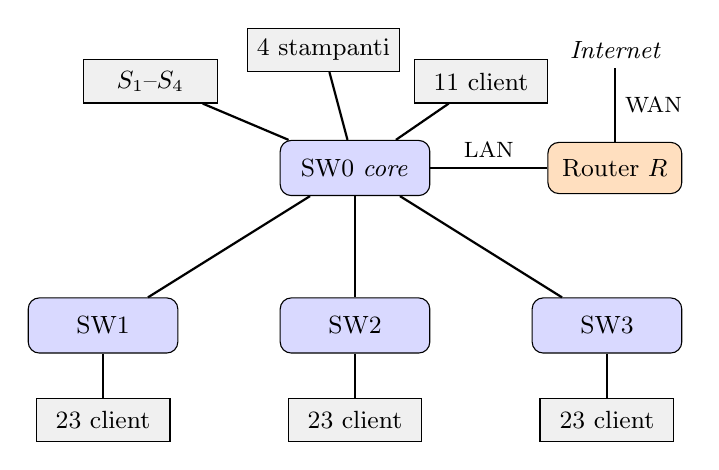
\begin{tikzpicture}[font=\small,
  sw/.style={draw,fill=blue!15,rounded corners,minimum width=1.9cm,minimum height=0.7cm},
  dev/.style={draw,fill=gray!12,minimum width=1.7cm,minimum height=0.55cm},
  rt/.style={draw,fill=orange!25,rounded corners,minimum width=1.7cm,minimum height=0.65cm},
  l/.style={thick}]
  % core, router, internet
  \node[sw] (core) at (0,0) {SW0 \textit{core}};
  \node[rt] (R) at (3.3,0) {Router $R$};
  \node (inet) at (3.3,1.5) {\itshape Internet};
  \draw[l] (R) -- (inet) node[midway,right]{\footnotesize WAN};
  \draw[l] (core) -- (R) node[midway,above]{\footnotesize LAN};
  % servers, printers, residual clients on core
  \node[dev] (srv) at (-2.6,1.1) {$S_1$--$S_4$};
  \node[dev] (prn) at (-0.4,1.5) {4 stampanti};
  \node[dev] (c0)  at (1.6,1.1) {11 client};
  \draw[l] (core) -- (srv);
  \draw[l] (core) -- (prn);
  \draw[l] (core) -- (c0);
  % access switches
  \node[sw] (a1) at (-3.2,-2) {SW1};
  \node[sw] (a2) at (0,-2)    {SW2};
  \node[sw] (a3) at (3.2,-2)  {SW3};
  \draw[l] (core) -- (a1);
  \draw[l] (core) -- (a2);
  \draw[l] (core) -- (a3);
  % clients
  \node[dev] (d1) at (-3.2,-3.2) {23 client};
  \node[dev] (d2) at (0,-3.2)    {23 client};
  \node[dev] (d3) at (3.2,-3.2)  {23 client};
  \draw[l] (a1) -- (d1);
  \draw[l] (a2) -- (d2);
  \draw[l] (a3) -- (d3);
\end{tikzpicture}
\end{center}
Ripartizione: \emph{core} $=$ router $+$ 4 server $+$ 4 stampanti $+$ 11 client
$=20$ porte device $+\,3$ uplink $=23$ porte; ogni switch d'accesso $=23$ client
$+\,1$ uplink $=24$ porte. Totale client $11+3\cdot23 = 80$; totale device $89$.

\medskip
\noindent\textbf{a) Cavi minimi per non avere partizioni.}
\[
\underbrace{89}_{\text{device}\to\text{switch}} \;+\;
\underbrace{3}_{\text{link inter-switch }(k-1)} \;=\; \boxed{92\ \text{cavi}} .
\]
I 3 link inter-switch sono il \textbf{minimo spanning} (albero): bastano per la
connettività senza partizioni, senza link ridondanti (la robustezza ai guasti qui
è data dalla topologia a stella, non da cavi extra). Il cavo $R\to$ Internet (lato
WAN) è separato: $+1$ se lo si conta.

\medskip
\noindent\textbf{b) Servizi indispensabili.}
\begin{itemize}
\item \textbf{DHCP} -- assegna automaticamente a 80+ host indirizzo IP, maschera,
\emph{default gateway} e server DNS (a mano sarebbe ingestibile).
\item \textbf{DNS} -- risoluzione nome\,$\to$\,IP, senza cui la navigazione di
fatto non funziona.
\end{itemize}
La traduzione degli indirizzi verso Internet (NAT/PAT) è invece compito del
\textbf{router $R$}, non dei server.

\medskip
\noindent\textbf{c) WAN $=$ \texttt{129.1.255.254}: rispetta le linee guida?}
Come \emph{forma} sì: in \texttt{129.1.0.0/16} il broadcast è \texttt{129.1.255.255}
e l'ultimo host valido è proprio \texttt{129.1.255.254} (regola ``router $=$ ultimo
indirizzo utile''). \emph{Ma} quella linea guida riguarda l'interfaccia
\textbf{interna (LAN)}, cioè il default gateway degli host locali: qui
\texttt{129.1.255.254} è sull'interfaccia \textbf{WAN}, su una rete pubblica esterna
e tipicamente imposta dall'ISP, quindi non è ad essa che la regola della rete
locale si applica. Coincidenza di forma, ma criterio non pertinente.

\medskip
\noindent\textbf{d) Tutti gli host in Internet con un solo IP pubblico.}
\textbf{NAT/PAT} (\emph{Port Address Translation}, IP masquerading) sul router: la
LAN usa indirizzi \textbf{privati} (es.\ \texttt{10.0.0.0/8} o
\texttt{192.168.0.0/16}) e $R$ traduce \emph{molti-a-uno} tutte le connessioni
uscenti sull'unico IP pubblico \texttt{129.1.255.254}, distinguendo i flussi col
numero di porta. Così 80+ host condividono un solo indirizzo pubblico.
\end{solution}

\dfn{Metodo (progettazione fisica con switch a $p$ porte)}{
1) conta le \textbf{porte device} $D$ (client $+$ server $+$ stampanti $+$
interfaccia LAN del router);
2) numero minimo di switch ad albero: $pk-2(k-1)\ge D \Rightarrow
k\ge\frac{D-2}{p-2}$;
3) topologia a \textbf{stella} (core $+$ accessi), mai a catena, per isolare i
guasti; client distribuiti uniformemente per il carico;
4) \textbf{cavi minimi senza partizioni} $= D + (k-1)$ (device $+$ uplink di un
albero, nessun link ridondante).
}


%==================================================================
\chapter{Congestione e bilanciamento del carico}
%==================================================================

\section{Router con due link in uscita e instradamento probabilistico}

\begin{Exercise}{Scritto -- 8 router verso Router 1, split casuale}{congestione-router}
8 router spediscono $Y$ pkt/s al Router~1. Ogni pacchetto ha dimensione $K$
kilobit. Dal Router~1 escono \textbf{due link}: il \emph{link superiore} viene
scelto con probabilità $\alpha=50\%$, il \emph{link inferiore} con probabilità
$1-\alpha$. Il \textbf{link inferiore} ha capacità massima $X\cdot K$ kilobit/s.
\begin{enumerate}
\item[a)] In quale caso il Router~1 sarà \emph{di certo} congestionato? Spiegare.
\item[b)] Qual è il limite sulla dimensione di $Y$ (con $\alpha=50\%$) per non
creare congestione?
\end{enumerate}
\footnotesize($X=$ somma delle due cifre meno significative \emph{non nulle} della
matricola; $K=$ prodotto delle stesse due cifre. Es.\ cifre $e=4,\,f=5$:
$X=4+5=9$, $K=4\cdot5=20$.)
\end{Exercise}

\begin{solution}
\textbf{Passo 0 -- modello.} Una porta d'uscita di un router è una \emph{coda}: i
pacchetti arrivano con un certo ritmo (\emph{rate} d'arrivo $\lambda$) e vengono
trasmessi al ritmo massimo consentito dalla capacità del link (\emph{rate} di
servizio $\mu$). La condizione di stabilità (niente congestione) è
\[
\rho = \frac{\lambda}{\mu} \le 1
\qquad\Longleftrightarrow\qquad
\text{carico offerto} \le \text{capacità del link}.
\]
Se $\lambda > \mu$ la coda cresce \textbf{senza limite}: è la congestione.

\medskip
\textbf{Passo 1 -- traffico entrante (in bit/s).} Gli 8 router immettono ciascuno
$Y$ pkt/s, quindi
\[
\lambda_{\text{in}} = 8Y \ \text{pkt/s} = 8Y\cdot K \ \text{kbit/s}.
\]

\textbf{Passo 2 -- come si divide sui due link.} L'instradamento è \emph{casuale
per-pacchetto}: una frazione $\alpha$ va sopra, $1-\alpha$ va sotto. I rate
\emph{medi} offerti ai due link sono quindi
\[
\lambda_{\text{sup}} = \alpha\cdot 8YK, \qquad
\lambda_{\text{inf}} = (1-\alpha)\cdot 8YK .
\]
Con $\alpha=50\%$ ciascun link riceve \emph{in media} metà del traffico:
\[
\lambda_{\text{sup}} = \lambda_{\text{inf}} = \tfrac{1}{2}\cdot 8YK = 4YK \ \text{kbit/s}.
\]

\medskip
\noindent\textbf{a) Quando è \emph{di certo} congestionato.}
Del link \emph{inferiore} conosciamo la capacità ($\mu_{\text{inf}}=XK$ kbit/s),
quindi è l'unico su cui possiamo dare una risposta \emph{certa} (la capacità del
link superiore non è data). Il link inferiore va in congestione quando il carico
medio che gli arriva supera la sua capacità:
\[
\boxed{(1-\alpha)\cdot 8YK > XK}
\qquad\Longleftrightarrow\qquad
(1-\alpha)\cdot 8Y > X .
\]
Notare che $K$ si semplifica: la dimensione del pacchetto non conta, conta il
\emph{ritmo}. Con $\alpha=50\%$ diventa $4Y > X$, cioè
\[
Y > \frac{X}{4}.
\]

\emph{Perché ``di certo''.} Lo split è probabilistico, quindi istante per istante
la frazione sul link inferiore oscilla. \textbf{Ma} su tanti pacchetti (legge dei
grandi numeri) la frazione converge a $1-\alpha$ con probabilità $1$: se quel
valore medio supera la capacità, la coda della porta cresce illimitatamente
\emph{con certezza}. È diverso dal ``potrebbe congestionarsi'' dovuto ai burst:
anche sotto soglia, una raffica sfortunata di pacchetti tutti verso lo stesso link
crea code \emph{temporanee}, ma non una congestione \emph{permanente}. La
congestione certa è una questione di \textbf{medie}, i burst sono una questione di
\textbf{varianza}.

\medskip
\noindent\textbf{b) Limite di $Y$ con $\alpha=50\%$ per non congestionare.}
Serve carico medio sul link inferiore $\le$ capacità:
\[
4YK \le XK
\qquad\Longleftrightarrow\qquad
\boxed{\,Y \le \dfrac{X}{4}\ \text{pkt/s}\,}.
\]
(Con $\alpha=50\%$ i due link portano lo stesso carico medio $4YK$: il vincolo
stringente è quello del link di cui conosciamo la capacità, l'inferiore. Se il
link superiore avesse capacità $\ge XK$, $Y\le X/4$ basta per entrambi.)

\medskip
\noindent\textbf{Verifica numerica} (cifre $e=4,\,f=5 \Rightarrow X=9,\ K=20$).
Capacità link inferiore $=XK = 180$ kbit/s. Limite $Y_{\max}=X/4 = 2{,}25$ pkt/s.
A $Y=2{,}25$: entrante $8\cdot2{,}25 = 18$ pkt/s $= 360$ kbit/s, divisi metà e metà
$\Rightarrow 180$ kbit/s su ciascun link $=$ \emph{esattamente} la capacità
(al limite). Per $Y>2{,}25$ il link inferiore è di certo congestionato.

\medskip
\textbf{Nota -- stretto o largo?} In un modello a fluido la soglia è $Y\le X/4$. In
una coda \emph{stocastica} reale (arrivi a raffica), già a $\rho=1$ il ritardo
medio diverge: per starsene tranquilli serve $\rho<1$ strettamente, cioè
$Y<X/4$ con un piccolo margine.
\end{solution}

\dfn{Metodo (congestione di una porta d'uscita)}{
1) porta tutto in \textbf{bit/s} (rate $=$ pkt/s $\times$ bit/pkt);
2) carico medio sul link $=$ (frazione di traffico instradata) $\times$ (traffico
totale entrante);
3) \textbf{niente congestione} $\Leftrightarrow$ carico medio $\le$ capacità del
link ($\rho=\lambda/\mu\le1$);
4) \textbf{congestione certa} $\Leftrightarrow$ carico medio $>$ capacità (la coda
cresce illimitatamente, per la legge dei grandi numeri, a prescindere dai singoli
lanci di moneta);
5) i \emph{burst} (varianza) danno code temporanee anche sotto soglia, ma non
congestione permanente.
}


%==================================================================
\chapter{Diagnostica e comandi di rete}
%==================================================================

\section{Interpretazione dell'output di \texttt{ping}}

\begin{Exercise}{Scritto 2024-05-31, n.\ 1 --- PING a flora.cs.unibo.it}{ping-2024}
Il comando \texttt{ping flora.cs.unibo.it} produce il risultato seguente: quale
può essere la causa? E quali protocolli/servizi di rete vengono usati per produrre
i risultati indicati?
\begin{center}
\ttfamily\footnotesize
\begin{tabular}{@{}l@{}}
\hline
PING flora.cs.unibo.it (130.136.5.36): 56 data bytes \\
64 bytes from 130.136.5.36: icmp\_seq=0 ttl=54 time=16.624 ms \\
64 bytes from 130.136.5.36: icmp\_seq=1 ttl=54 time=15.590 ms \\
ping: sendto: No route to host \\
ping: sendto: No route to host \\
Request timeout for icmp\_seq 2 \\
Request timeout for icmp\_seq 3 \\
64 bytes from 130.136.5.36: icmp\_seq=4 ttl=54 time=15.404 ms \\
64 bytes from 130.136.5.36: icmp\_seq=5 ttl=54 time=14.712 ms \\
\hline
\end{tabular}
\end{center}
E se invece il risultato fosse stato questo?
\begin{center}
\ttfamily\footnotesize
\begin{tabular}{@{}l@{}}
\hline
PING flora.cs.unibo.it: cannot resolve flora.cs.unibo.it: Unknown host \\
\hline
\end{tabular}
\end{center}
\end{Exercise}

\begin{solution}
\textbf{Come funziona \texttt{ping} (i protocolli in gioco).}
\begin{enumerate}
\item \textbf{DNS} (applicazione, UDP porta 53): prima cosa, il \emph{nome}
\texttt{flora.cs.unibo.it} viene risolto nell'indirizzo IP
\texttt{130.136.5.36}. Il fatto che la prima riga mostri già l'IP tra parentesi
dimostra che \textbf{la risoluzione DNS è andata a buon fine}.
\item \textbf{ICMP} (livello Rete, dentro IP): \texttt{ping} invia messaggi
\emph{ICMP Echo Request} e attende gli \emph{ICMP Echo Reply}. Da qui vengono
\texttt{icmp\_seq} (numero di sequenza), \texttt{time} (RTT andata+ritorno) e
\texttt{ttl} del pacchetto di risposta.
\item \textbf{IP} per instradare i datagrammi, e \textbf{ARP} (livello Link) per
trovare il MAC del next-hop (gateway) sulla LAN locale.
\end{enumerate}
\emph{Lettura del \texttt{ttl=54}:} le risposte partono da un TTL iniziale tipico
(64) e perdono $1$ per ogni router attraversato $\Rightarrow 64-54 = \mathbf{10}$
hop circa fino a \texttt{flora}. Il TTL costante ($54$) e i tempi quasi uguali
($\sim15$ ms) sui ping riusciti dicono che \textbf{il percorso è sempre lo stesso}.

\medskip
\noindent\textbf{Primo caso --- causa.} Il DNS funziona (l'IP c'è) e i ping
\texttt{seq} 0,1,4,5 tornano regolari; in mezzo, \texttt{seq} 2,3 falliscono con
\texttt{No route to host} / \texttt{Request timeout}. Il messaggio
\texttt{No route to host} è un \textbf{ICMP Destination Unreachable -- Host
Unreachable} (tipo 3): un router del cammino (o l'host stesso) per quei pacchetti
non aveva una rotta valida. Essendo il guasto \textbf{intermittente} (passa, non
passa, ripassa sullo stesso percorso), la causa è un \textbf{problema transitorio
di instradamento/raggiungibilità}: un router o un link lungo il cammino
temporaneamente giù, instradamento instabile (\emph{route flapping} con
riconvergenza del protocollo di routing) o next-hop momentaneamente irraggiungibile.
\emph{Non} è un problema di DNS (il nome è stato risolto) né del server
\texttt{flora} (quando il percorso c'è, risponde regolarmente).

\medskip
\noindent\textbf{Secondo caso --- causa.} Qui \texttt{ping} non arriva nemmeno a
spedire l'ICMP: si ferma prima, alla \textbf{risoluzione del nome}.
\texttt{cannot resolve \dots Unknown host} $=$ \textbf{fallimento DNS}: server DNS
irraggiungibile / non configurato, oppure il nome non esiste (nessun record A),
oppure DNS mal configurato sull'host. Il problema è quindi a livello di
\textbf{servizio DNS}, non di connettività verso \texttt{flora}: senza l'IP,
\texttt{ping} non può costruire l'Echo Request.
\end{solution}

\dfn{Diagnostica con \texttt{ping}: cosa guardare}{
\textbf{Catena:} nome $\xrightarrow{\text{DNS/UDP 53}}$ IP
$\xrightarrow{\text{ICMP Echo in IP}}$ risposta.
\begin{itemize}
\item Compare l'IP tra parentesi $\Rightarrow$ \textbf{DNS OK}; \texttt{cannot
resolve / Unknown host} $\Rightarrow$ \textbf{DNS KO} (ci si ferma qui).
\item \texttt{No route to host} $=$ ICMP \emph{Host Unreachable} $\Rightarrow$
problema di \textbf{routing/raggiungibilità} (se intermittente: percorso
instabile).
\item \texttt{Request timeout} $=$ nessuna risposta entro il timeout (pacchetto
perso o host/firewall che scarta).
\item \texttt{ttl} risposta $=$ TTL\_iniziale (64/128/255) $-$ n.\ hop
$\Rightarrow$ stima la distanza; \texttt{time} $=$ RTT.
\end{itemize}
}


%==================================================================
\chapter{Crittografia}
%==================================================================

\dfn{Notazione}{
$\Ks{A}$ = chiave privata di Alice, $\Kp{A}$ = pubblica di Alice (idem $B,C$);
$\HASH(\cdot)$ = funzione hash; $\Ks{X}[\cdot]$ = firma (cifra con la privata);
$\Kp{X}[\cdot]$ = cifratura con la pubblica. \textbf{Principio:} l'asimmetrico
tocca solo cose piccole (l'hash o una chiave di sessione), mai il messaggio
grande.
}

\begin{Exercise}{Scritto 2020-09-14, n.\ 4}{cr-2020}
Alice spedisce a Bob un messaggio $M$ con garanzia di mittente e privacy.
Inoltre Alice pretende da Bob la prova che il messaggio ricevuto non possa
essere in seguito ripudiato (Bob non può dire di non averlo ricevuto o di averlo
ricevuto diverso). Realizzare lo schema di cifratura.
\end{Exercise}

\begin{solution}
\begin{align*}
\text{Alice}\to\text{Bob:}\quad & C=\Kp{B}\big[\,M,\ \Ks{A}(\HASH(M))\,\big]\\
\text{Bob:}\quad & \Ks{B}(C)\to M,\text{firma};\quad \Kp{A}(\text{firma})\overset{?}{=}\HASH(M)\\
\text{Bob}\to\text{Alice (ACK):}\quad & \Ks{B}\big[\,\HASH(M)\,\big]
\end{align*}
\begin{itemize}
\item \textbf{Mittente}: firma $\Ks{A}(\HASH(M))$ verificata con $\Kp{A}$.
\item \textbf{Privacy}: cifratura con $\Kp{B}$ $\Rightarrow$ solo Bob legge.
\item \textbf{Non ripudio della ricezione}: l'ACK firmato da Bob
($\Ks{B}[\HASH(M)]$, verificabile con $\Kp{B}$) prova ad Alice che Bob ha
ricevuto \emph{proprio} $M$. \emph{Questo giro di ritorno è il cuore
dell'esercizio.}
\end{itemize}
\end{solution}

\begin{Exercise}{Scritto 2021-01-14, n.\ 4}{cr-2021}
Alice spedisce a Bob $M1$ \textbf{molto grande} con garanzia di non
ripudiabilità (no privacy). Bob risponde con $m2$ \textbf{piccolo} con garanzia
di mittente, privacy e non-Replay (solo Alice lo legge, una sola volta, e da
Bob). Schema di costo minimo.
\end{Exercise}

\begin{solution}
\begin{align*}
\text{Alice}\to\text{Bob:}\quad & M1,\ \Ks{A}(\HASH(M1)),\ R \quad(\text{$R$ nonce fresco})\\
\text{Bob verifica:}\quad & \Kp{A}(\text{firma})\overset{?}{=}\HASH(M1)\\
\text{Bob}\to\text{Alice:}\quad & c=\Kp{A}\big[\,m2,\ R,\ \Ks{B}(\HASH(m2,R))\,\big]\\
\text{Alice:}\quad & \Ks{A}(c)\to m2,R,\text{firma};\ \Kp{B}(\text{firma})\overset{?}{=}\HASH(m2,R);\ R\overset{?}{=}\text{atteso}
\end{align*}
\begin{itemize}
\item $M1$ grande $\Rightarrow$ si firma l'\textbf{hash} (non $M1$) e si manda in
chiaro: non ripudiabilità + efficienza.
\item $m2$: mittente ($\Ks{B}$) + privacy ($\Kp{A}$, asimmetrico diretto perché
piccolo) + non-Replay (nonce $R$).
\end{itemize}
\textbf{Nota:} la sola $c=\Kp{A}(\Ks{B}(m2))$ dà mittente+privacy ma resta
\emph{ri-giocabile}; il nonce $R$ chiude il non-Replay.
\end{solution}

\begin{Exercise}{Scritto 2022-06-10, n.\ 3}{cr-2022}
Alice $\to$ Bob: $M1$ \textbf{molto grande}, solo non ripudiabilità (no privacy,
tutti possono leggere). Bob $\to$ Alice: $m2$ \textbf{piccolo} con mittente,
privacy e non-Replay. Schema di costo minimo.
\end{Exercise}

\begin{solution}
Identico per struttura all'esercizio~\ref{cr-2021}:
\begin{align*}
\text{Alice}\to\text{Bob:}\quad & M1,\ \Ks{A}(\HASH(M1)),\ R\\
\text{Bob}\to\text{Alice:}\quad & \Kp{A}\big[\,m2,\ R,\ \Ks{B}(\HASH(m2,R))\,\big]
\end{align*}
$M1$ in chiaro con firma sull'hash (non ripudio + efficienza); risposta cifrata
per Alice, firmata da Bob, con nonce per il non-Replay.
\end{solution}

\begin{Exercise}{Scritto 2023-05-26, n.\ 4}{cr-2023}
Alice manda $m1$ a Bob e $m2$ a Charlie; poi Bob e Charlie se li scambiano, così
entrambi hanno $m1$ e $m2$. Garanzie: confidenzialità (Trudy non legge),
mittente (è Alice), integrità. In che modo Trudy può \emph{ancora} attaccare?
\end{Exercise}

\begin{solution}
Idea: Alice \textbf{firma} ogni messaggio (mittente+integrità end-to-end) e si
cifra \textbf{per ogni destinatario}; la firma viaggia col messaggio e
sopravvive all'inoltro.
\begin{align*}
\text{Alice}\to\text{Bob:}\quad & \Kp{B}\big[\,m1,\ \Ks{A}(\HASH(m1))\,\big]\\
\text{Alice}\to\text{Charlie:}\quad & \Kp{C}\big[\,m2,\ \Ks{A}(\HASH(m2))\,\big]\\
\text{Bob}\to\text{Charlie:}\quad & \Kp{C}\big[\,m1,\ \Ks{A}(\HASH(m1))\,\big]\\
\text{Charlie}\to\text{Bob:}\quad & \Kp{B}\big[\,m2,\ \Ks{A}(\HASH(m2))\,\big]
\end{align*}
Confidenzialità (cifratura per destinatario), mittente+integrità (firma di Alice
verificabile da entrambi). Bob non può manomettere $m1$: la firma non tornerebbe.

\medskip
\textbf{Attacchi residui di Trudy} (le garanzie non includono la freschezza):
\begin{itemize}
\item \textbf{Replay}: nessun nonce/timestamp $\Rightarrow$ Trudy reintroduce un
ciphertext valido e Bob lo riaccetta. (Fix: nonce dentro la busta firmata.)
\item \textbf{Cancellazione/DoS}: confidenzialità$\ne$disponibilità; Trudy può
bloccare i pacchetti.
\item \textbf{Analisi del traffico}: la cifratura nasconde il contenuto, non i
metadati (chi$\to$chi, quando, quanto).
\end{itemize}
\end{solution}

\begin{Exercise}{Scritto 2023-07-21, n.\ 4}{cr-2023b}
Alice invia $N$ messaggi segreti $m_1\dots m_N$ (brevi) a Bob; $N$ non è noto a
priori e Alice deve segnalare in modo affidabile l'ultimo. Bob deve ricevere
tutto in modo privato (anche $N$ deve restare segreto) e sicuro (nessuno
modifichi contenuto, ordine o numero; può ritardare/aggiungere/duplicare ma non
cancellare). Definire il protocollo.
\end{Exercise}

\begin{solution}
Per ogni pacchetto $i$ (reali $1\dots N$, più \textbf{decoy} $i>N$):
\[
P_i=\Kp{B}\big[\ m_i,\ i,\ \texttt{flag\_ultimo},\ \Ks{A}\big(\HASH(m_i,i,\texttt{flag\_ultimo})\big)\ \big]
\]
Alice continua a spedire decoy (dummy firmati) anche \emph{dopo} $N$.

\medskip
\textbf{Bob:} decifra con $\Ks{B}$ e verifica la firma di Alice (scarta tutto ciò
che non è firmato $\Rightarrow$ blocca iniezioni/duplicati forgiati); ordina per
$i$, scarta i duplicati; al pacchetto con \texttt{flag\_ultimo} sa che $N$ è la
fine; poiché Trudy non può cancellare, prima o poi ha tutti gli $1\dots N$;
scarta i pacchetti con numero $>N$.

\medskip
\begin{tabularx}{\linewidth}{lX}
\hline
Attacco di Trudy & Difesa \\
\hline
Leggere contenuto & cifratura $\Kp{B}$ \\
Dedurre $N$ contando i pacchetti & decoy $>N$ + flag ``ultimo'' cifrato \\
Modificare contenuto/numero/ordine & firma $\Ks{A}(\HASH(m_i,i,\dots))$ \\
Iniettare pacchetti & non ha $\Ks{A}$ $\Rightarrow$ firma non valida \\
Duplicare & numero di sequenza già visto \\
Riordinare & Bob riordina per $i$ \\
Fine anticipata fittizia & flag ``ultimo'' firmato, non forgiabile \\
Ritardare & tempo finito $\Rightarrow$ arrivano tutti \\
\hline
\end{tabularx}
\end{solution}

\begin{Exercise}{Scritto 2024-05-31, n.\ 2}{cr-2024}
Alice e Bob si scambiano 4 numeri primi (tra 1 e 100): $a_1,a_2$ da Alice a Bob
e $b_1,b_2$ da Bob ad Alice. Serve garanzia del mittente e integrità; il
prodotto finale $X=a_1\cdot a_2\cdot b_1\cdot b_2$ deve essere noto a entrambi ma
non a Trudy (privacy), resistendo a forza bruta e replay.
\end{Exercise}

\begin{solution}
Lo spazio dei valori è piccolo: cifrare un numero con $\Kp{}$ in modo
deterministico è attaccabile per forza bruta (Trudy cifra tutti i candidati e
confronta). Si aggiunge quindi un \textbf{nonce/sale casuale} $R$ dentro la busta:
\begin{align*}
\text{Alice}\to\text{Bob:}\quad & \Kp{B}\big[\,a_1,a_2,\ R_A,\ \Ks{A}(\HASH(a_1,a_2,R_A))\,\big]\\
\text{Bob}\to\text{Alice:}\quad & \Kp{A}\big[\,b_1,b_2,\ R_B,\ \Ks{B}(\HASH(b_1,b_2,R_B))\,\big]
\end{align*}
Ognuno verifica la firma (mittente+integrità) e la freschezza del nonce
(non-Replay). Entrambi calcolano $X=a_1 a_2 b_1 b_2$. Trudy non vede mai i
fattori (cifrati) $\Rightarrow$ non conosce $X$; il sale casuale $R$ rende i
ciphertext non indovinabili nonostante il piccolo spazio dei valori
(anti-forza-bruta).
\end{solution}

\begin{Exercise}{Scritto 2025-05-30, n.\ 4}{cr-2025}
Schema efficiente per spedire da Alice a Bob un messaggio $M$ \textbf{molto
grande} con non ripudiabilità e non falsificazione (no confidenzialità), con
contromisure al replay. La chiave pubblica di Alice è ottenuta via CA fidata.
\end{Exercise}

\begin{solution}
\begin{align*}
\text{Alice}\to\text{Bob:}\quad & M,\ T,\ \Ks{A}\big(\HASH(M,T)\big)\\
\text{Bob:}\quad & \Kp{A}(\text{firma})\overset{?}{=}\HASH(M,T);\quad T\ \text{fresco?}
\end{align*}
\begin{itemize}
\item $M$ grande $\Rightarrow$ si firma l'\textbf{hash} e si manda $M$ in chiaro
(no privacy richiesta) $\Rightarrow$ efficiente.
\item \textbf{Non ripudio / non falsificazione}: firma con $\Ks{A}$, verificata
con $\Kp{A}$ (autentica perché ottenuta via CA fidata).
\item \textbf{Anti-replay}: timestamp (o nonce) $T$ incluso nell'hash firmato;
Bob accetta solo se fresco.
\end{itemize}
\end{solution}


%==================================================================
\chapter{Wireless e Modulazione Digitale}
%==================================================================

\dfn{Link Budget --- formula generale}{
Ogni componente del percorso radio contribuisce in dB (si sommano algebricamente):
\[
  P_{rx}\ [\text{dBm}] = P_{tx}\ [\text{dBm}] + G_{tx}\ [\text{dBi}] + G_{rx}\ [\text{dBi}] - \text{PL}\ [\text{dB}]
\]
La comunicazione è possibile se e solo se $P_{rx} \geq RS$ (Receiver Sensitivity).
In condizioni meteo avverse si aggiunge un margine: $P_{rx} \geq RS + \text{FOM}$,
con $\text{FOM} \geq 10\ \text{dB}$ per nebbia/pioggia.

\medskip
\textbf{Path loss free-space (formula in miglia):}
\[
  \text{PL} = 36.6 + 20\log_{10}(f_{\text{MHz}}) + 20\log_{10}(d_{\text{mi}})
\]
\textbf{Regola dei 6 dB:} raddoppiare la distanza $\Rightarrow +6\ \text{dB}$ di path loss
($20\log_{10}2 \approx 6.02$).

\medskip
\textbf{Conversione mW $\leftrightarrow$ dBm:} $0\ \text{dBm}=1\ \text{mW}$;
ogni $+3\ \text{dB}$ raddoppia la potenza; ogni $+10\ \text{dB}$ la moltiplica
per 10. Esempio: $32\ \text{mW} = 2^5\ \text{mW} = +15\ \text{dBm}$.
}

\dfn{Modulazione digitale}{
\begin{center}
\begin{tabular}{lccc}
\hline
Schema & Simboli & bit/simbolo & Robustezza al rumore \\
\hline
BPSK  & 2  & 1 & massima \\
QPSK  & 4  & 2 & alta \\
8-PSK & 8  & 3 & media \\
QAM-16& 16 & 4 & media-bassa \\
QAM-64& 64 & 6 & bassa \\
\hline
\end{tabular}
\end{center}
\textbf{Bit rate} $= \text{Symbol Rate} \times \text{bit/simbolo}$.
Con OFDM, il bit rate totale è la somma dei contributi di tutti i sub-carrier:
$\text{Bit rate totale} = N_{\text{sub}} \times \text{SR} \times \text{bit/simbolo}$.
}

%------------------------------------------------------------------
\section{Modulazione e codifica digitale}
%------------------------------------------------------------------

\begin{Exercise}{Scritto 2021-01-14, n.\,1 --- QAM-16 vs QPSK}{wl-qam}
Che differenza c'è tra una codifica digitale QAM-16 e una QPSK?
\end{Exercise}

\begin{solution}
Entrambe sono \textbf{codifiche digitali} che mappano bit in simboli radio, ma differiscono
nel numero di simboli e nei parametri del segnale che fanno variare.

\medskip
\textbf{QPSK (Quadrature Phase Shift Keying):}
\begin{itemize}
  \item 4 simboli $\Rightarrow$ 2 bit/simbolo.
  \item Varia \emph{solo la fase} dell'onda portante: $0°,90°,180°,270°$.
  \item L'ampiezza rimane costante $\Rightarrow$ il segnale è molto robusto al rumore
        di ampiezza (che è la forma più comune di interferenza radio).
\end{itemize}

\textbf{QAM-16 (Quadrature Amplitude Modulation, 16 simboli):}
\begin{itemize}
  \item 16 simboli $\Rightarrow$ 4 bit/simbolo (il doppio di QPSK).
  \item Varia \emph{sia la fase che l'ampiezza}: costellazione $4\times4$.
  \item Trasmette il doppio dei bit per simbolo, ma i 16 punti della costellazione
        sono più vicini fra loro $\Rightarrow$ più sensibile al rumore, serve un
        link budget migliore a parità di distanza.
\end{itemize}

\textbf{In sintesi:} QPSK offre maggiore \emph{robustezza} (meno errori in canali
rumorosi), QAM-16 offre maggiore \emph{efficienza spettrale} (più bit per simbolo).
La scelta dipende dalla qualità del canale disponibile.
\end{solution}

\begin{Exercise}{Scritto 2023-07-21, n.\,6 --- QPSK e matrice di parità}{wl-qpsk-par}
Ragionando solo a livello fisico, se si trasmette un file da 16~Mbit su un canale
radio a frequenza singola (narrowband) con QPSK e Symbol Rate pari a
500\,000~Sym/sec:
\begin{enumerate}
  \item quanto impiega la trasmissione?
  \item e se si usasse una \emph{matrice di parità} $16\times16$ per contrastare
        1 bit errato in media ogni 256 bit trasmessi?
\end{enumerate}
\end{Exercise}

\begin{solution}
\textbf{Parte 1 --- senza parità.}

QPSK $\Rightarrow$ 2 bit/simbolo.
\[
  \text{Bit rate} = 500\,000\ \tfrac{\text{sym}}{\text{s}} \times 2\ \tfrac{\text{bit}}{\text{sym}}
                 = 1\,000\,000\ \text{bit/s} = 1\ \text{Mbps}
\]
\[
  T = \frac{16\,000\,000\ \text{bit}}{1\,000\,000\ \text{bit/s}} = \boxed{16\ \text{s}}
\]

\medskip
\textbf{Parte 2 --- con matrice di parità $16\times16$.}

Una matrice di parità $16\times16$ consente di correggere 1 bit errato ogni $16\times16=256$
bit di dati. Come funziona:
\begin{itemize}
  \item Si prendono 256 bit di dati, li si dispongono in una matrice $16\times16$.
  \item Si aggiungono \textbf{16 bit di parità per le righe} + \textbf{16 bit per le colonne}
        $= 32$ bit di overhead ogni 256 bit utili.
  \item Il totale da trasmettere per ogni blocco: $256 + 32 = 288$ bit.
\end{itemize}

Overhead ratio: $\tfrac{288}{256}$.

Bit totali da trasmettere per il file:
\[
  16\,000\,000 \times \frac{288}{256} = 16\,000\,000 \times 1.125 = 18\,000\,000\ \text{bit}
\]
\[
  T = \frac{18\,000\,000}{1\,000\,000} = \boxed{18\ \text{s}}
\]

Il tempo aumenta del 12.5\% rispetto al caso senza parità, ma si ottiene la
capacità di \emph{correggere} (non solo rilevare) 1 bit errato per blocco da 256.
\end{solution}

\begin{Exercise}{Scritto 2023-07-21, n.\,10 --- Encoding K}{wl-encK}
Un sistema di comunicazione wireless usa la seguente codifica (Encoding~K) a
3 bit per simbolo (8 simboli totali). La tabella associa ogni tripletta di bit a
una forma d'onda con riferimento $A\sin(Bt)$:

\begin{center}
\begin{tabular}{cl}
\hline
Simbolo (3 bit) & Forma d'onda \\
\hline
\texttt{011} & anticipo di fase (early) \\
\texttt{001} & anticipo di fase (early) \\
\texttt{000} & segnale di riferimento $A\sin(Bt)$ \\
\texttt{010} & ritardo di fase (late) \\
\texttt{111} & anticipo di fase --- ampiezza $2A$ \\
\texttt{101} & riferimento --- ampiezza $2A$ \\
\texttt{100} & ritardo di fase (late) \\
\texttt{110} & ritardo di fase --- ampiezza $2A$ \\
\hline
\end{tabular}
\end{center}

(a) Quali sono i 18 bit trasmessi per la sequenza esadecimale \texttt{0EAF}\ldots
    (completare a 18 bit con zero a destra)?\\
(b) Quali simboli (triplette) corrispondono?\\
(c) Descrivere le forme d'onda generate.
\end{Exercise}

\begin{solution}
\textbf{(a) Conversione esadecimale $\to$ binario:}
\[
  \underbrace{\texttt{0}}_{\texttt{0000}}
  \underbrace{\texttt{E}}_{\texttt{1110}}
  \underbrace{\texttt{A}}_{\texttt{1010}}
  \underbrace{\texttt{F}}_{\texttt{1111}}
  +\underbrace{\texttt{00}}_{\text{padding}}
  \;=\;
  \texttt{00 0011 1010 1011 1100}
\]

Sequenza completa (18 bit):
\[
  \texttt{000011101010111100}
\]

\medskip
\textbf{(b) Raggruppamento in simboli da 3 bit:}
\[
  \underbrace{\texttt{000}}_{s_1}\ \underbrace{\texttt{011}}_{s_2}\ \underbrace{\texttt{101}}_{s_3}\ \underbrace{\texttt{010}}_{s_4}\ \underbrace{\texttt{111}}_{s_5}\ \underbrace{\texttt{100}}_{s_6}
\]

\medskip
\textbf{(c) Forme d'onda per i 6 simboli:}
\begin{center}
\begin{tabular}{cll}
\hline
Simbolo & Forma d'onda & Descrizione \\
\hline
\texttt{000} & $A\sin(Bt)$         & riferimento (fase zero, ampiezza $A$) \\
\texttt{011} & $A\sin(Bt+\phi)$    & anticipo di fase (early), ampiezza $A$ \\
\texttt{101} & $2A\sin(Bt)$        & riferimento ampiezza $2A$ \\
\texttt{010} & $A\sin(Bt-\phi)$    & ritardo di fase (late), ampiezza $A$ \\
\texttt{111} & $2A\sin(Bt+\phi)$   & anticipo di fase, ampiezza $2A$ \\
\texttt{100} & $A\sin(Bt-\phi)$    & ritardo di fase (late), ampiezza $A$ \\
\hline
\end{tabular}
\end{center}

Questo schema combina variazione di \textbf{fase} (anticipo/ritardo/$0°$) e
\textbf{ampiezza} ($A$ o $2A$): è una forma di \textbf{ASK+PSK} (simile a QAM),
con 8 simboli = 3 bit/simbolo.
\end{solution}

\begin{Exercise}{Scritto 2024-05-31, n.\,2 --- Modulazione e interferenza}{wl-interf}
Quali tra le tecniche di modulazione digitale (FSK, ASK, PSK, QAM) nelle reti
senza fili sono \textbf{meno} resistenti all'interferenza (cioè a più rischio di
errori)? Giustificare la risposta.
\end{Exercise}

\begin{solution}
La risposta è \textbf{ASK} (Amplitude Shift Keying), ed è la meno robusta.

\medskip
\textbf{Perché ASK è vulnerabile?}
Il rumore elettromagnetico tipico in un canale radio agisce principalmente
sull'\textbf{ampiezza} del segnale (attenuazioni, riflessioni, interferenze da
altri trasmettitori). ASK codifica l'informazione proprio nell'ampiezza: una
variazione di ampiezza dovuta al rumore viene letta come un simbolo diverso
$\Rightarrow$ errore di decodifica.

\medskip
\textbf{Confronto con gli altri schemi:}
\begin{itemize}
  \item \textbf{FSK} --- varia la \emph{frequenza}: il rumore di ampiezza non
        cambia la frequenza $\Rightarrow$ molto robusto.
  \item \textbf{PSK} --- varia la \emph{fase}: il rumore di ampiezza non
        cambia la fase $\Rightarrow$ molto robusto (QPSK è lo standard WiFi).
  \item \textbf{QAM} --- varia sia ampiezza che fase $\Rightarrow$ più efficiente
        di PSK ma meno robusto, perché la componente ASK della modulazione resta
        vulnerabile; comunque più robusto dell'ASK puro.
\end{itemize}

\textbf{Ordine crescente di robustezza:} ASK $<$ QAM $<$ PSK $\approx$ FSK.
\end{solution}

%------------------------------------------------------------------
\section{Link Budget e propagazione}
%------------------------------------------------------------------

\begin{Exercise}{Scritto 2021-01-14, n.\,2 --- Link budget da figura}{wl-lb2021}
Quale è il link budget di un sistema come quello in figura? Il sistema può
comunicare? Perché?

\medskip
\emph{(La figura nel testo originale riporta: Ptx, guadagni di entrambe le antenne
e la Receiver Sensitivity del ricevitore. Applicare il metodo sotto.)}
\end{Exercise}

\begin{solution}
Il metodo è sempre lo stesso:
\[
  \text{Link Budget} = P_{tx} + G_{tx} + G_{rx} - \text{PL}
\]
Si confronta con la Receiver Sensitivity RS:
\begin{itemize}
  \item Se $\text{LB} \geq RS$ $\Rightarrow$ \textbf{il sistema comunica}.
  \item Se $\text{LB} < RS$ $\Rightarrow$ \textbf{il segnale è sotto soglia}, non comunica.
\end{itemize}

Il path loss si calcola con la formula free-space (se non specificato altrimenti):
$\text{PL} = 36.6 + 20\log_{10}(f_{\text{MHz}}) + 20\log_{10}(d_{\text{mi}})$.

\medskip
\emph{Nota: la figura specifica del testo d'esame è necessaria per ricavare i
valori numerici esatti. Il procedimento rimane identico a quello degli esercizi
seguenti.}
\end{solution}

\begin{Exercise}{Scritto 2024-05-31, n.\,3 --- Regola dei 6\,dB}{wl-6db}
Cosa indica la regola dei 6\,dB e quale utilità pratica ha?
\end{Exercise}

\begin{solution}
\textbf{Enunciato:} raddoppiare la distanza tra trasmettitore e ricevitore causa
un aumento di $\approx6\ \text{dB}$ nel path loss (attenuazione).

\medskip
\textbf{Dimostrazione} dal path loss free-space:
\[
  \Delta\text{PL} = 20\log_{10}(2d) - 20\log_{10}(d) = 20\log_{10}(2) \approx 20 \times 0.301 = 6.02\ \text{dB}
\]

\textbf{Conseguenza simmetrica:} dimezzare la distanza $\Rightarrow -6\ \text{dB}$
di path loss (il link budget migliora di 6\,dB).

\medskip
\textbf{Utilità pratica:} invece di ricalcolare il path loss dall'inizio con la
formula logaritmica, si può stimare rapidamente l'effetto di uno spostamento.
Esempi:
\begin{itemize}
  \item Ho un link budget di $+10\ \text{dB}$ a 100\,m; a 200\,m sarà $+4\ \text{dB}$
        (ancora funzionante, ma con meno margine).
  \item Se il sistema funziona a 500\,m con FOM$=0$, raddoppiando a 1000\,m serve
        $+6\ \text{dBm}$ di potenza (o $+6\ \text{dBi}$ di guadagno antenna) per
        mantenere la stessa qualità.
\end{itemize}
\end{solution}

\begin{Exercise}{Scritto 2022-06-10, n.\,7 --- Comunicazione a 5 miglia, nebbia e zona di Fresnel}{wl-5mi}
Un sistema di comunicazione wireless deve supportare comunicazione su distanza
di 5 miglia ($1\ \text{miglio}=1.609\ \text{km}$) a frequenza 1.9\,GHz. Le due
antenne non hanno ostruzioni della zona di Fresnel e hanno entrambe guadagno
$+7\ \text{dBi}$; la receiver sensitivity è $RS=-97\ \text{dBm}$.
\begin{enumerate}
  \item Quale potenza trasmissiva (in mW) serve per una comunicazione affidabile
        anche in una giornata di nebbia?
  \item È possibile spostare i due dispositivi a distanza doppia mantenendo la
        stessa comunicazione?
  \item A quanto ammonta il raggio della zona di Fresnel al 100\%
        (in metri; $1\ \text{feet}=30.5\ \text{cm}$)?
\end{enumerate}
\end{Exercise}

\begin{solution}
\textbf{Parte 1 --- Potenza minima (con nebbia, FOM $\geq 10\ \text{dB}$).}

Step 1: calcolo del path loss.
\begin{align*}
  \text{PL} &= 36.6 + 20\log_{10}(1900) + 20\log_{10}(5) \\
            &= 36.6 + 65.6 + 14.0 = 116.2\ \text{dB}
\end{align*}

Step 2: potenza ricevuta in funzione di $P_{tx}$.
\[
  P_{rx} = P_{tx} + 7 + 7 - 116.2 = P_{tx} - 102.2\ \text{dBm}
\]

Step 3: condizione con margine nebbia ($\text{FOM}=10\ \text{dB}$).
\[
  P_{rx} \geq RS + 10 \implies P_{tx} - 102.2 \geq -97 + 10
  \implies P_{tx} \geq 15.2\ \text{dBm}
\]

Step 4: conversione dBm $\to$ mW (metodo additivo, $+3\ \text{dB} = \times 2$).
\[
  15\ \text{dBm} = 0\ \text{dBm} + \underbrace{3+3+3+3+3}_{5\ \text{raddoppi}}
  \implies 1\ \text{mW} \times 2^5 = \boxed{32\ \text{mW}}
\]

\medskip
\textbf{Parte 2 --- Distanza doppia (regola dei 6\,dB).}

Raddoppiare la distanza $\Rightarrow +6\ \text{dB}$ di path loss $\Rightarrow$
FOM si riduce: $10 - 6 = +4\ \text{dB}$.

Poiché $+4\ \text{dB} > 0$, il segnale ricevuto è ancora \emph{sopra} la soglia
RS $\Rightarrow$ \textbf{sì, è ancora possibile comunicare}. Rimane però solo
4\,dB di margine (invece di 10), quindi la comunicazione è meno robusta.

\medskip
\textbf{Parte 3 --- Raggio zona di Fresnel al 100\%.}

Formula empirica:
\[
  r_{100\%} = 72.2 \times \sqrt{\frac{d_{\text{mi}}}{4 \cdot f_{\text{GHz}}}}
            = 72.2 \times \sqrt{\frac{5}{4 \times 1.9}}
            = 72.2 \times \sqrt{0.658}
            = 72.2 \times 0.811
            \approx 58.6\ \text{feet}
\]

Conversione: $58.6 \times 0.305\ \text{m/foot} \approx \boxed{17.9\ \text{m}}$.

\emph{Attenzione: un refuso comune è scrivere ``cm'' invece di ``m''; il risultato
corretto è quasi 18 \textbf{metri}.}

\medskip
\textbf{Interpretazione della zona di Fresnel:} è l'ellissoide attorno alla linea
diretta trasmettitore--ricevitore all'interno del quale il segnale radio è
significativo. Se un ostacolo penetra nel 60\% di questo raggio, il segnale
si degrada. Le antenne erano indicate senza ostruzione $\Rightarrow$ nessuna
perdita aggiuntiva da ostruzione Fresnel.
\end{solution}

\begin{Exercise}{Scritto 2023-05-26, n.\,6 --- OFDM e scelta dello schema PSK}{wl-ofdm}
Se un canale radio OFDM ha 18 sub-carrier e un symbol rate di 500\,000
simboli/sec, quanti simboli della codifica digitale PSK deve adottare per
riuscire a trasferire un file da 54\,Mbit in non più di 4 secondi,
\textbf{massimizzando la resistenza all'errore di canale}? Quanto tempo
impiega esattamente?
\end{Exercise}

\begin{solution}
\textbf{Bit rate totale del canale OFDM:}
\[
  \text{SR}_{\text{totale}} = 18\ \text{sub-carrier} \times 500\,000\ \tfrac{\text{sym}}{\text{s}}
  = 9\,000\,000\ \text{sym/s}
\]

\textbf{Bit rate minimo necessario per consegnare 54\,Mbit in 4\,s:}
\[
  R_{\min} = \frac{54\,000\,000\ \text{bit}}{4\ \text{s}} = 13\,500\,000\ \text{bit/s}
\]

\textbf{Quanti bit per simbolo servono almeno?}
\[
  b \geq \frac{13\,500\,000}{9\,000\,000} = 1.5\ \text{bit/simbolo}
\]

Quindi serve almeno $b=2$ bit/simbolo $\Rightarrow$ BPSK ($b=1$) non basta.

\textbf{Massimizzare resistenza all'errore} = usare il \emph{minor numero possibile
di simboli} che soddisfi il requisito (meno simboli = punti più distanti nella
costellazione = meno errori).

$\Rightarrow$ si sceglie \textbf{QPSK} ($b=2$, 4 simboli), il minimo sufficiente.

\medskip
\textbf{Bit rate effettivo con QPSK:}
\[
  R = 9\,000\,000 \times 2 = 18\,000\,000\ \text{bit/s}
\]

\textbf{Tempo di trasferimento:}
\[
  T = \frac{54\,000\,000}{18\,000\,000} = \boxed{3\ \text{s}}
\]

Il file viene consegnato in 3 secondi (dentro il limite di 4).
\end{solution}

\begin{Exercise}{Scritto 2023-05-26, n.\,10 --- Link budget con tabella di bitrate}{wl-lb2023}
Un sistema wireless ha le prestazioni del ricevitore indicate in tabella:
\begin{center}
\begin{tabular}{cc}
\hline
Bitrate nominale & Link Budget minimo \\
\hline
1~Mbps  &  5~dB \\
2~Mbps  &  8~dB \\
4~Mbps  & 14~dB \\
8~Mbps  & 20~dB \\
16~Mbps & 26~dB \\
32~Mbps & 32~dB \\
64~Mbps & 38~dB \\
\hline
\end{tabular}
\end{center}
Trasmettitore: $P_{tx}=25\ \text{mW}$, antenna $+8\ \text{dBi}$; ricevitore:
antenna omnidirezionale $+3\ \text{dBi}$; path loss a 1 miglio: $-80\ \text{dB}$;
$RS = -75\ \text{dBm}$.
\begin{enumerate}
  \item A quale velocità avviene la comunicazione?
  \item E se la distanza si riducesse a $\tfrac{1}{3}$ di miglio?
\end{enumerate}
\end{Exercise}

\begin{solution}
\textbf{Parte 1 --- distanza 1 miglio.}

Step 1: conversione $P_{tx}=25\ \text{mW} \to \text{dBm}$.
\[
  10\ \text{mW} = 10\ \text{dBm}, \quad
  20\ \text{mW} = 13\ \text{dBm}, \quad
  25\ \text{mW} \approx 14\ \text{dBm}
\]
(precisamente: $10\log_{10}25 = 13.98 \approx 14\ \text{dBm}$).

Step 2: Link Budget $= P_{rx} - RS$, ovvero il margine sopra la soglia.
\[
  P_{rx} = 14 + 8 + 3 - 80 = -55\ \text{dBm}
\]
\[
  \text{LB} = P_{rx} - RS = -55 - (-75) = +20\ \text{dB}
\]

Step 3: dalla tabella, $\text{LB}=20\ \text{dB}$ corrisponde a $\boxed{8\ \text{Mbps}}$.

\medskip
\textbf{Parte 2 --- distanza $\tfrac{1}{3}$ di miglio.}

La variazione di path loss rispetto a 1 miglio è:
\[
  \Delta\text{PL} = 20\log_{10}\!\left(\tfrac{1/3}{1}\right) = 20\log_{10}\!\left(\tfrac{1}{3}\right)
  = -20 \times 0.477 = -9.54\ \text{dB}
\]
(il path loss \emph{diminuisce} di $9.54\ \text{dB}$ a distanza più corta).

Nuovo link budget:
\[
  \text{LB}_{\text{new}} = 20 + 9.54 \approx +29.5\ \text{dB}
\]

Dalla tabella: $29.5\ \text{dB}$ soddisfa il requisito per 16\,Mbps (26\,dB)
ma non per 32\,Mbps (32\,dB) $\Rightarrow$ $\boxed{16\ \text{Mbps}}$.
\end{solution}

\begin{Exercise}{Scritto 2025-05-30, n.\,10 --- Guadagno antenna per 40\,Mbps}{wl-gain2025}
Un sistema wireless trasmette con $\text{IRPO}=20\ \text{mW}$ e un decadimento
dovuto alla distanza pari a $-110\ \text{dB}$. Il ricevitore ha le seguenti
sensitivity:
\begin{center}
\begin{tabular}{cc}
\hline
Receiver Sensitivity & Bitrate nominale \\
\hline
$-96\ \text{dBm}$ & 10~Mbps \\
$-93\ \text{dBm}$ & 20~Mbps \\
$-87\ \text{dBm}$ & 40~Mbps \\
$-82\ \text{dBm}$ & 80~Mbps \\
\hline
\end{tabular}
\end{center}
Quale guadagno totale (somma delle due antenne) è necessario per sostenere
almeno 40\,Mbps?
\end{Exercise}

\begin{solution}
\textbf{Target:} $\geq 40\ \text{Mbps}$, che richiede $P_{rx} \geq RS_{40} = -87\ \text{dBm}$.

Step 1: $P_{tx}$ in dBm.
\[
  20\ \text{mW} = 10\ \text{mW} \times 2 = 10\ \text{dBm} + 3\ \text{dBm} = 13\ \text{dBm}
\]

Step 2: equazione del link budget con $G = G_{tx}+G_{rx}$ incognito.
\[
  P_{rx} = P_{tx} + G + \text{PL} = 13 + G - 110 = G - 97
\]

Step 3: imporre $P_{rx} \geq -87$.
\[
  G - 97 \geq -87 \implies G \geq +10\ \text{dBi}
\]

$\boxed{G_{tx}+G_{rx} \geq 10\ \text{dBi}}$. Se le due antenne sono identiche,
bastano $5\ \text{dBi}$ ciascuna.

\medskip
\emph{Verifica:} con $G=10$: $P_{rx} = 13 + 10 - 110 = -87\ \text{dBm}$,
esattamente la soglia per 40\,Mbps $\checkmark$.
\end{solution}

%------------------------------------------------------------------
\section{Propagazione e multipath}
%------------------------------------------------------------------

\begin{Exercise}{Scritto 2022-06-10, n.\,8 --- Interferenza multipath}{wl-mpath}
Un segnale radio a $37.5\ \text{MHz}$ percorre una distanza di 29\,m in linea
retta (LoS). Lo stesso segnale percorre 21\,m prima di rimbalzare di 90° e poi
raggiunge il ricevitore.
\begin{enumerate}
  \item Il segnale rimbalzato arriva in anticipo o in ritardo di fase rispetto al
        segnale LoS?
  \item La risultante dei due segnali consente una buona comunicazione?
        Motivare con i calcoli.
  \item Se la potenza fosse di 20\,mW, di quanto andrebbe aumentata per garantire
        un'ottima comunicazione?
\end{enumerate}
\end{Exercise}

\begin{solution}
\textbf{Parte 1 --- percorso del segnale rimbalzato.}

Il segnale parte dal trasmettitore T, percorre 21\,m fino al punto di rimbalzo B,
poi gira di 90° verso il ricevitore R. La geometria forma un triangolo retto
con angolo retto in B:
\[
  TB = 21\ \text{m}, \quad TR = 29\ \text{m} \quad (\text{LoS})
\]
Per il teorema di Pitagora:
\[
  BR = \sqrt{TR^2 - TB^2} = \sqrt{29^2 - 21^2} = \sqrt{841-441} = \sqrt{400} = 20\ \text{m}
\]
Percorso rimbalzato totale: $21 + 20 = 41\ \text{m}$.

Percorso \textbf{più lungo} di quello LoS $\Rightarrow$ il segnale rimbalzato
arriva \textbf{in ritardo di fase} rispetto al segnale LoS.

\medskip
\textbf{Parte 2 --- interferenza costruttiva o distruttiva?}

Differenza di percorso: $\Delta d = 41 - 29 = 12\ \text{m}$.

Lunghezza d'onda:
\[
  \lambda = \frac{c}{f} = \frac{3\times10^8\ \text{m/s}}{37.5\times10^6\ \text{Hz}} = 8\ \text{m}
\]

Differenza di percorso in lunghezze d'onda:
\[
  \frac{\Delta d}{\lambda} = \frac{12}{8} = 1.5\ \lambda
\]

Decomposizione: $1.5\,\lambda = 1\,\lambda + 0.5\,\lambda$. La parte intera ($1\,\lambda$)
è un giro completo $\Rightarrow$ non cambia la fase. La parte $0.5\,\lambda$
corrisponde a \textbf{180° di sfasamento}.

Conclusione: i due segnali arrivano al ricevitore \textbf{in opposizione di fase}.
Avendo percorso simile e quindi ampiezza simile, si \textbf{annullano}
$\Rightarrow$ \textbf{no, non consente buona comunicazione}.

\medskip
\textbf{Parte 3 --- aumentare la potenza aiuta?}

\textbf{No}, nessun aumento di potenza risolve il problema. Aumentando $P_{tx}$,
entrambi i segnali (LoS e rimbalzato) crescono proporzionalmente e la loro
\emph{differenza di fase rimane 180°}. La somma continua a essere vicino a zero
indipendentemente dall'ampiezza. L'interferenza distruttiva è dovuta alla
geometria (differenza di percorso), non alla potenza.

L'unica soluzione è cambiare la posizione delle antenne (modificare $\Delta d$)
o usare antenne con diverso puntamento per sopprimere il percorso di rimbalzo.
\end{solution}

%------------------------------------------------------------------
\section{Protocolli MAC wireless}
%------------------------------------------------------------------

\begin{Exercise}{Scritto 2025-05-30, n.\,6 --- Vulnerabilità del frame in CSMA/CA}{wl-vuln}
Spiegare il concetto di \textbf{vulnerabilità del frame} in protocolli MAC ad
accesso casuale in reti senza fili.
\end{Exercise}

\begin{solution}
In un protocollo ad accesso casuale, una collisione avviene quando due stazioni
trasmettono \emph{contemporaneamente} sullo stesso canale. Il \textbf{periodo di
vulnerabilità} è la finestra temporale durante la quale una trasmissione in corso
può essere distrutta da un'altra trasmissione che inizia.

\medskip
\textbf{Confronto Ethernet (CSMA/CD) vs.\ 802.11 (CSMA/CA):}

\begin{center}
\begin{tabular}{p{0.2\linewidth}p{0.35\linewidth}p{0.35\linewidth}}
\hline
 & \textbf{Ethernet / CSMA/CD} & \textbf{WiFi 802.11 / CSMA/CA} \\
\hline
Rilevazione collisione & SÌ: la stazione sente il canale \emph{mentre} trasmette
  (collision detection) & NO: in radio non si può sentire il proprio segnale
  durante la trasmissione (half-duplex) \\
Periodo vulnerabile & Solo il tempo di propagazione $\tau$
  (molto breve, $\sim\mu$s) & L'intero tempo di trasmissione del frame \\
\hline
\end{tabular}
\end{center}

\medskip
In wireless il \textbf{periodo di vulnerabilità} è uguale alla
\textbf{durata del frame}: se un'altra stazione inizia a trasmettere
in qualsiasi momento durante la trasmissione corrente, il frame è
irrimediabilmente corrotto e deve essere ritrasmesso per intero.

\medskip
\textbf{Conseguenza:} i frame più lunghi sono più vulnerabili (più lunga è la
finestra $\Rightarrow$ più probabile che qualcuno trasmetta nel mezzo).

\medskip
\textbf{Mitigazione con RTS/CTS:} prima di inviare un frame lungo si trasmettono
i frame corti RTS (\emph{Request To Send}) e CTS (\emph{Clear To Send}).
Il ``periodo vulnerabile'' si riduce alla durata dell'RTS (piccolo), invece
dell'intero frame dati. Le stazioni vicine che sentono il CTS si mettono in
silenzio per la durata dell'intera trasmissione.
\end{solution}

\end{document}
